\chapter{Ingeniería de Software Ágil}

\section{Proceso de desarrollo}

Hacer agilidad no nos asegura calidad. Para ello primero hay que asegurarse de hacer ingeniería de software además de agilidad. Hay diferentes procesos de ingeniería o ciclos de vida y podemos tomar el siguiente: descubrimiento y definición de requerimientos (Discovery \& Requirements), análisis y diseño (Analysis \& Design), implementación y pruebas (Implementation \& Testing), integración y pruebas (Integration \& Testing), despliegue (Delivery) y "operación y monitoreo" (Operation \& Monitoring). En la última fase se contempla operaciones, monitoreo y el análisis de datos. Operaciones en cuanto a aseguramiento de la operatividad y rendimiento del software. El monitoreo de datos es el seguimiento a determinadas acciones que podemos cuantificar y que nos arrojaran datos relevantes para la estrategia (KPIs). Y el análisis de datos es la base de la optimización de la estrategia, que nos permite modificar, continuar o establecer nuevas directrices, sin perder de vista el objetivo final del software o producto.

\begin{figure}[h]
  \centering
  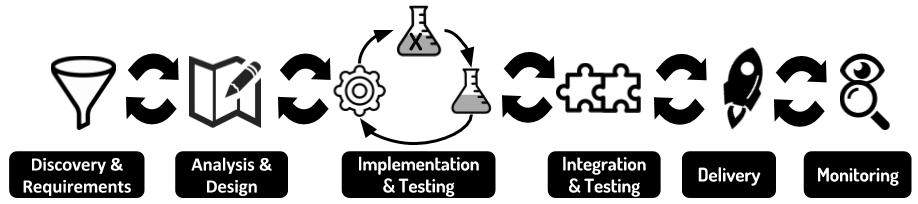
\includegraphics[width=0.99\textwidth]{PhasesOfSoftwareEngineering}
  \caption{Ciclo de ingeniería de Software}
  \centering
  \label{fig:PhasesOfSoftwareEngineering} %\ref{fig:PhasesOfSoftwareEngineering}
\end{figure}
\FloatBarrier % Command to control the position of floating images. With its, I can get the figures not to be pushed to the end of the document.
% El comando FloatBarrier es usado aqui para que la imagen se clave en este lugar y que no sea acarreada al final del documento.


Dicho esto, hay que considerar que el proceso de ingeniería de software ágil se hace sobre piezas de software (batch, feature o historia de usuario), y si bien es secuencial, tiene las fases del ciclo de vida que se solapan con las de otros piezas (ver fig. \ref{fig:PhasesOfSoftwareEngineering}). Es decir que el software se va desarrollando de a fragmentos o pequeñas piezas de software, en forma incremental y evolutiva. Cada pieza de software se desarrolla con diferentes instancias del ciclos de vida.

Correr este proceso bajo un marco ágil como Scrum, con prácticas ágiles es lo que podemos llamar ingeniería de software ágil (Agile Software Engineering). Además es conveniente introducir la idea de prácticas continuas, es decir refinamiento continuo (análisis y diseño con trabajo UX continuo), testing continuo (continuous testing), integración continua (continuous integration), despliegue o entrega continua (continuous deployment \& continuous delivery) y monitoreo continuo (continuous monitoring). 
Dicho esto, tenemos que tener en cuenta cómo unir y ajustar el proceso de ingeniería de software con el marco de trabajo Scrum. En este sentido es que se plantea ejecutar las fases del proceso de ingeniería, sobre historias de usuario, dentro del tren de sprints. En un equipo extremadamente autónomo y ágil, todas las fases se pueden desarrollar bajo el tren de sprints de Scrum.

\begin{figure}[h]
  \centering
  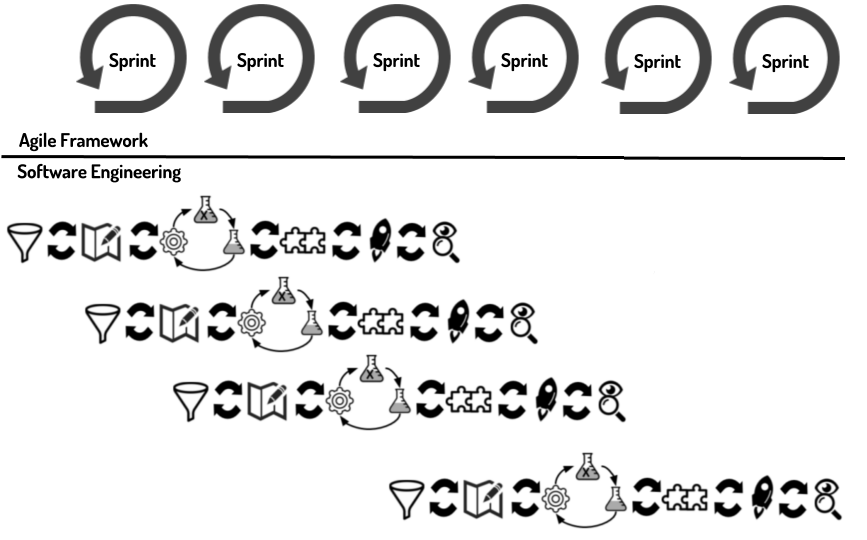
\includegraphics[width=0.99\textwidth]{AgileSoftwareEngineering}
  \caption{Ingeniería de Software Ágil}
  \centering
  \label{fig:AgileSoftwareEngineering} %\ref{fig:AgileSoftwareEngineering}
\end{figure}
\FloatBarrier % Command to control the position of floating images. With its, I can get the figures not to be pushed to the end of the document.
% El comando FloatBarrier es usado aqui para que la imagen se clave en este lugar y que no sea acarreada al final del documento.

De este modo, se integra el testing en fases más tempranas del desarrollo, por lo que QA no retrasa al equipo de desarrollo, porque QA está dentro del equipo y se trabaja con testing continuo. Los mismo sucede con UX y Operaciones.

\section{Testing continuo}

Si pensamos en Agile Testing pensamos en que queremos un testing dentro del equipo, con todo el equipo colaborando, que no sea solo una fase en un cascada, que reduzca el tiempo para recibir retroalimentación y asegure calidad suficiente. Cuando se incorpora agile testing, se introducen algunas prácticas, como por ejemplo Testing de “todo el equipo”, integración continua, testing guiado por pruebas (TDD), desarrollo guiado por pruebas de aceptación (ATDD), implementar la V de calidad usando historias, entre otros. 

\begin{figure}[h]
  \centering
  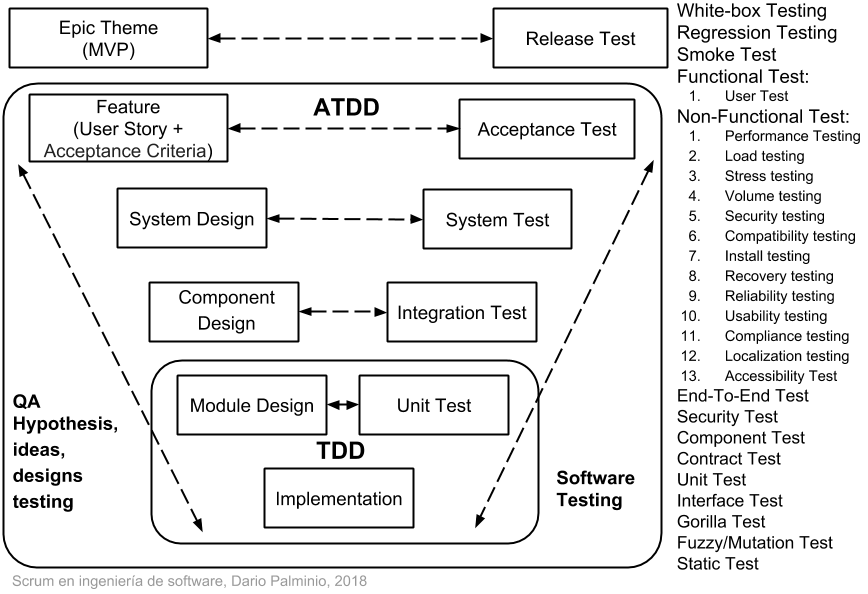
\includegraphics[width=0.99\textwidth]{AgileTesting_V}
  \caption{Modelo en V de calidad y testing}
  \centering
  \label{fig:AgileTesting_V} %\ref{fig:AgileTesting_V}
\end{figure}
\FloatBarrier % Command to control the position of floating images. With its, I can get the figures not to be pushed to the end of the document.
% El comando FloatBarrier es usado aqui para que la imagen se clave en este lugar y que no sea acarreada al final del documento.

Aunque considero que lo más importante es incorporar la mentalidad de testing continuo, independientemente de las prácticas o técnicas particulares.

\begin{figure}[h]
  \centering
  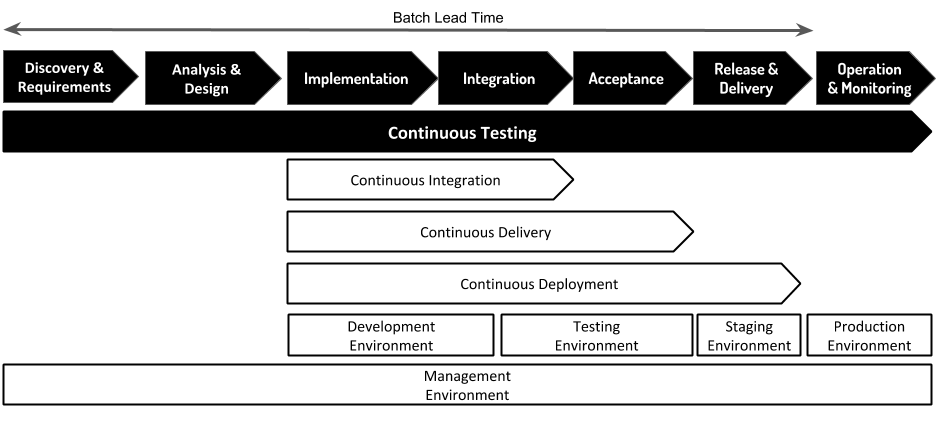
\includegraphics[width=0.99\textwidth]{structure_of_software_engineering_on_batch_life_cycle}
  \caption{Ciclo de vida de una historia y prácticas}
  \centering
  \label{fig:structure_of_software_engineering_on_batch_life_cycle} %\ref{fig:structure_of_software_engineering_on_batch_life_cycle}
\end{figure}
\FloatBarrier % Command to control the position of floating images. With its, I can get the figures not to be pushed to the end of the document.
% El comando FloatBarrier es usado aqui para que la imagen se clave en este lugar y que no sea acarreada al final del documento.

Cada fase del ciclo de vida del desarrollo puede contener prácticas de testing, desde las fases más tempranas hasta producción.

\begin{figure}[h]
  \centering
  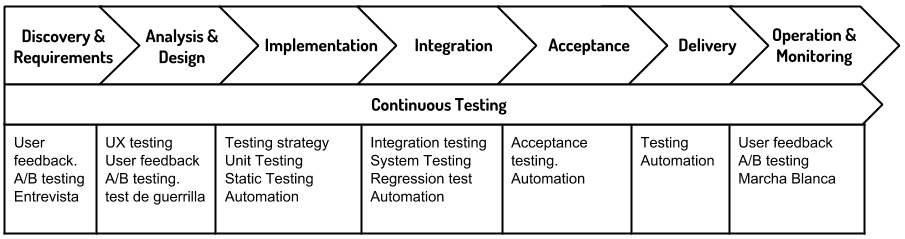
\includegraphics[width=0.99\textwidth]{continuous_testing_on_batch_life_cycle}
  \caption{Prácticas básicas en continuous testing}
  \centering
  \label{fig:continuous_testing_on_batch_life_cycle} %\ref{fig:continuous_testing_on_batch_life_cycle}
\end{figure}
\FloatBarrier % Command to control the position of floating images. With its, I can get the figures not to be pushed to the end of the document.
% El comando FloatBarrier es usado aqui para que la imagen se clave en este lugar y que no sea acarreada al final del documento.

Y, si lo pensamos bien, podemos decir que Scrum es una prueba de integración del sistema organizacional para validar continuamente si es posible que una organización entregue valor en un Sprint\footnote{Stacia Heimgartner Viscardi, Professional ScrumMaster's Handbook}. La prueba de Scrum revela los fallos de la organización, disfuncionalidades o los impedimentos que luego debemos buscar solucionar para lograr la agilidad organizacional. De este modo, cada Sprint que hagamos será un ciclo de testing organizacional, tanto de nuestro equipo como del resto de la organización, para levantar acciones de mejora que podemos explicitar, definir y evaluar en las sesiones de retrospectivas que tengamos y que apuntan a mejorar la propuesta de valor y el tiempo entre que se crea una historia y que la misma pueda ser validada por el cliente en forma operativa. Como dijo Jon Kern (co-autor del Manifiesto Ágil), “Ágil es reducir la brecha entre actuar y recibir feedback”, que en el desarrollo de productos se traduce a reducir el Time to Market (desde la perspectiva de negocio) o reducir el Delivery Lead Time (desde la perspectiva de DevOps); y Scrum nos ayuda a testear y medir esa brecha para reducirla. Con Scrum buscamos entregar software de calidad, que aporte valor, lo más pronto que sea posible.

\subsection{Tamaños de Testing}

Y hacia el equipo, el Scrum Master debe ayudarlo a que encuentre su manera de hacer buen testing y de mejorarlo. No existe realmente una forma única. Tampoco un convención de nombres y tipos de prueba claras. Depende de diferentes autores y de cada equipo. El Scrum Master debe ayudar con eso. Un ejemplo de esquema es el que han usado equipos en Google. A los desarrolladores de Google les gusta tomar decisiones basadas en datos, en lugar de confiar en el instinto o en algo que no se puede medir y evaluar. Ellos, llegaron a un acuerdo sobre un conjunto de convenciones de nomenclatura basadas en datos para sus pruebas. Llamaron a sus pruebas: "pequeñas", "medianas" y "grandes" \footnote{Test Sizes by Simon Stewart, Google Testing Blog, Monday, December 13, 2010.}. 

\begin{figure}[h]
  \centering
  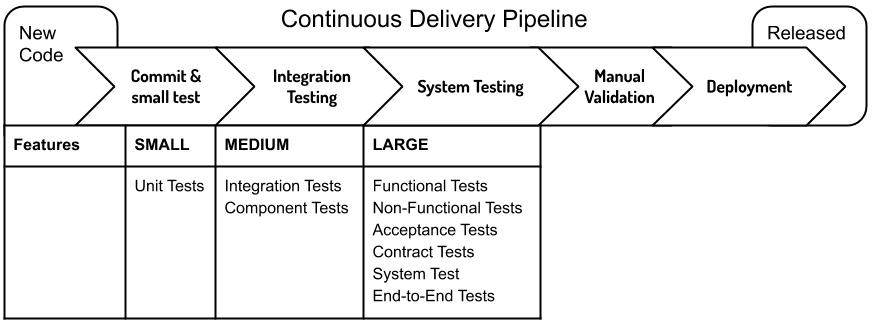
\includegraphics[width=0.99\textwidth]{Continuous_Delivery_Pipeline-small-medium-large}
  \caption{Tamaños de testing en el pipeline del Continuous Delivery}
  \centering
  \label{fig:Continuous_Delivery_Pipeline-small-medium-large} %\ref{fig:Continuous_Delivery_Pipeline-small-medium-large}
\end{figure}
\FloatBarrier % Command to control the position of floating images. With its, I can get the figures not to be pushed to the end of the document.
% El comando FloatBarrier es usado aqui para que la imagen se clave en este lugar y que no sea acarreada al final del documento.


Van de la prueba pequeña que equivale a una prueba de unidad, pasan por la prueba mediana que asegura que los niveles en la arquitectura de una aplicación pueden comunicarse correctamente y por una prueba grande que es una de extremo a extremo o de sistema.

\begin{figure}[h]
  \centering
  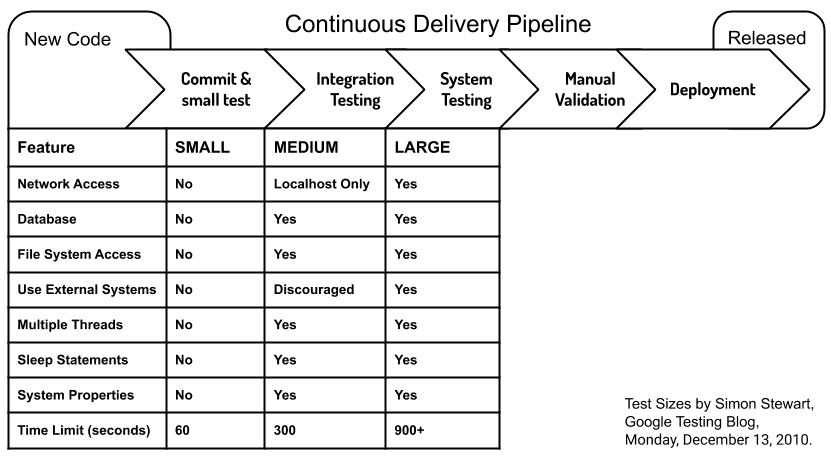
\includegraphics[width=0.99\textwidth]{TestingSize}
  \caption{Tamaños de testing y tipos en el pipeline del Continuous Delivery}
  \centering
  \label{fig:TestingSize} %\ref{fig:TestingSize}
\end{figure}
\FloatBarrier % Command to control the position of floating images. With its, I can get the figures not to be pushed to the end of the document.
% El comando FloatBarrier es usado aqui para que la imagen se clave en este lugar y que no sea acarreada al final del documento.


El Scrum Master debe asegurarse que el equipo encuentre la manera más efectiva y eficiente de hacer testing. Puede usar un esquema como el anterior, la pirámide de testing de Mike Cohn, la de Lisa Crispin o lo que encuentren apropiado. Sin testing de calidad no hay software de calidad.

\section{Prácticas técnicas}

Como ya he mencionado, es deseable que el SM vele por la excelencia técnica de su equipo y del proceso de desarrollo, buscando lograr un flujo limpio, cadenciosos y sostenible. Claro que la responsabilidad es del equipo y tanto un líder técnico como el SM, pueden liderar o guiar al equipo en el proceso de mejora continua del flujo de trabajo. Teniendo en cuenta las fases de desarrollo de los ítems de trabajo como historias, podemos tener dos aspectos en consideración para analizar el estado de nuestro procesos de desarrollo en cuanto a excelencia técnica. Por un lado, el aspecto de prácticas técnicas considerando la información, proceso, métodos, técnicas y organización (aquí se tiene en cuenta XP, DevOps, etc.). Por otro lado el aspecto tecnológico considerando las herramientas empleadas que cubren estas prácticas técnicas. Por ejemplo a continuación muestro un esquema de flujo y sus prácticas técnicas relacionadas.

\begin{figure}[h]
  \centering
  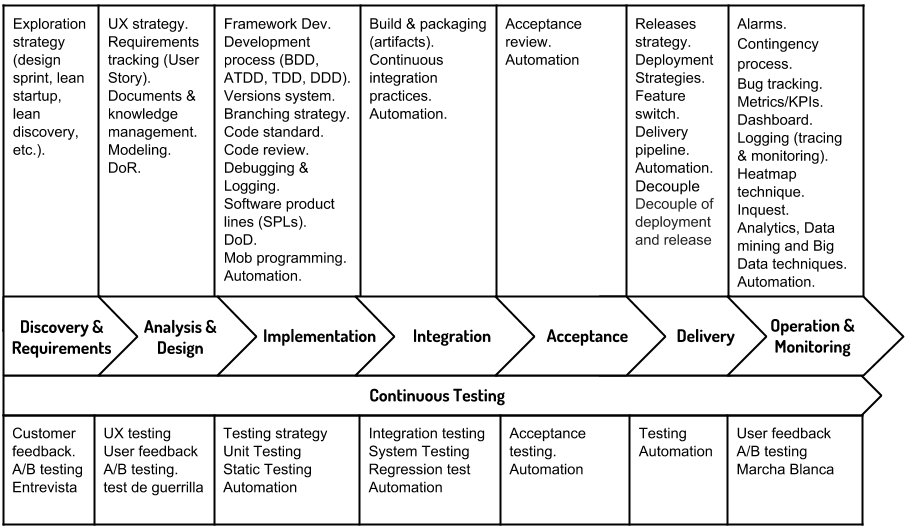
\includegraphics[width=0.99\textwidth]{practices_of_software_engineering}
  \caption{Flujo de prácticas técnicas}
  \centering
  \label{fig:practices_of_software_engineering} %\ref{fig:practices_of_software_engineering}
\end{figure}
\FloatBarrier % Command to control the position of floating images. With its, I can get the figures not to be pushed to the end of the document.
% El comando FloatBarrier es usado aqui para que la imagen se clave en este lugar y que no sea acarreada al final del documento.

Se puede hacer un esquema de flujo semejante con los aspecto tecnológico, de herramientas, correspondientes a cada fase.

Hay que tener en cuenta que para que el flujo de desarrollo de software fluya limpio y cadencioso, la experiencia del desarrollo debe ser memorable y fluida sobre una plataforma e infraestructura que la facilite. Es por esto que un equipo de desarrollo tiene interdependencia con equipos de operaciones e infraestructura y es parte del desafío de un equipo de alto rendimiento disminuir la brecha, empoderarse y facilitar la integración de ese área de conocimiento.

\begin{figure}[h]
  \centering
  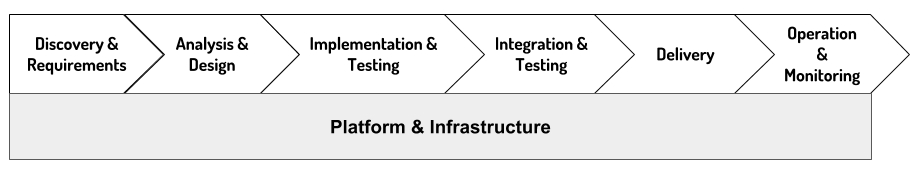
\includegraphics[width=0.99\textwidth]{Infrastructure}
  \caption{Plataforma e infraestructura}
  \centering
  \label{fig:Infrastructure} %\ref{fig:Infrastructure}
\end{figure}
\FloatBarrier % Command to control the position of floating images. With its, I can get the figures not to be pushed to the end of the document.
% El comando FloatBarrier es usado aqui para que la imagen se clave en este lugar y que no sea acarreada al final del documento.

\section{En síntesis}

Hacer ingeniería de software ágil es desarrollar software de valor, de modo iterativo, incremental y evolutivo, con un producto o servicio que evoluciona, donde los requisitos y soluciones cambian con el tiempo, haciendo entregas frecuentes de calidad y valor, testeando continuamente, con feedback rápido, trabajando con equipos auto-organizados y multidisciplinarios que mejoran, inmersos en un proceso compartido de toma de decisiones interactiva y dinámica y entendiendo el negocio. Y, lo más importante, es considerar que la ingeniería es, además de una práctica científica, una práctica humana. Construir software se trata de relaciones humanas en un sistema social. Por eso, hay que construir relaciones humanas de valor, que habiliten la entrega continua de valor. Según Patrick Lencioni, un equipo humano debería tener ciertas aptitudes funcionales que posibilitan el trabajo de alto rendimiento: confianza, sin miedo al conflicto, compromiso, asunción de responsabilidades y atención a los resultados. Según el proyecto Aristóteles de Google, la clave es la cultura del equipo y lo necesario en ella es la seguridad psicológica entendida como: el sentimiento de confianza de que el equipo no va a avergonzar, rechazar o castigar a alguien por sus opiniones, comportamientos o ideas. Y como un equipo no es una isla, la organización que le da contexto debe reforzar este tipo de cultura, el factor humano, para lograr personas extraordinarias desarrollando resultados extraordinarios.
